\chapter{De amaritudine in vita spirituali}
\begin{center}
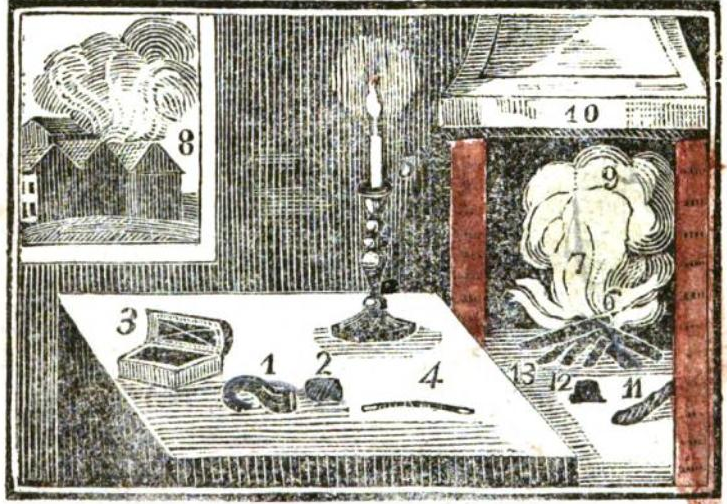
\includegraphics[scale=1.5]{Fire.png}
\end{center}

\section{Intended Audience}
This is intended for students who have completed Lectio 5 and 6 of Latin by the Natural Method and Chapter 5 of Lingua Latina Per Se Illustrata. There are 838 words in this chapter.

\section{Text}
Deinde Deus mīsit Eliseum in Caelum, mīsit eum in terrā. Deus deinde relinquit Eliseum Solum in terrā. Eliseus sōlus nōn scīvit locum in quō fuit. Deinde, Eliseus vīdit virum. Eliseus ambulāvit ad virum. Vir fuit prophēta Jēremīās. "Salvē" Eliseus dīxit ad eum "Quōmodo tē habēs?". "Bene valeō" dīxit Jēremīās, "Ut valēsne?" interrogāvit. "Male valeō" dīxit Eliseus. "Cūr?" Jēremīās interrogāvit. "Quia" inquit Eliseus "Nōn videō Deum, sīcut Vīdī eum". "Quārē trīstis es? Num scīs Deum in locīs omnibus esse?". "Sciō" respondit "Sed sī nōn videō eum, quōmodo laetificor?". "Sēde, faciō ignem." \par 
Jēremīās cēpit Chalybem. Cum chalybe in manū suā, pulsāvit silicem cum chalybe. Deinde ex silice scintilla volāvit in suscitābulum. In suscitābulō, fūmus ascendit in caelum. Deinde, Jēremīās posuit silicem et chalybem in terrā. Eliseus aspexit silicem et chalybem. Chalybs est dūrus est et etiam silex. Eliseus vīdit silicem quandō pater eius fēcit ignem in silvā. \par
Deinde Jēremīās ait Eliseō "Saepe, nōn sentīmus praesentiam Deī, et sentīmus sine eō". Jēremīās deinde cēpit suscitābulum, et ex sucitabūlō cēpit formitem. Fōmes fēcit fūmum, et Jēremīās posuit formitem in Turre Lignī. Flamma excitāvit. Fūmus ascendit ex lignō. Lignum ārdet. Eliseus posuit manum eius in lignō, et lignum ussit eum. "OOOW" exclāmāvit is. "Sīcut lignum ūrit manum tuam, absentia Deī ūrit animās nostrās. In ōrātiōne, nōn sentīmus. In labōre, nōn laetificāmur. In amōre Deī, cōnsōlātiō nōn invenītur.". "Quārē" dīxit Eliseus "Sī Deus sīcut flamma amōris est, dēbeō bonum sentīre". "Male dīcis" Jēremīās exclāmāvit "Scīsne Passiōnem Deī Nostram in Cruce, quandō amor vīvēns interfectus est?". "Ita" Eliseus ait "Sciō, sed tenebrae animī meī dolet mihi". \par
Subitō, Vestīmentum Elisēī ūrēbat. Eliseus iēcit id ex corpore suō. "Quārē accidit!?". "Deus dīligit tē cum permagnā amōre, Elisee" respondit Prophēta. "Sed incendium cēpit vestīmentum meum!", "Ita" Jēremīās ait "sīcut Fīlius Deī raptus est ex vīvō. Incendium cordis nostrī raptus est ex discipulīs eius". "Sed, in prīmō diē sabbatī, surrēxit cum magnā potestāte. Sīcut is, sīcut tū, sī dīligit eum". "Dīligō eum" dīxit Eliseus, "sed quārē pulsāvit mē?". "Quia", dīxit "Dēbēmus eum sōlum dīligere. Sī dīligis creātiōnem, dīligis eum nōn". \pār 
Ex Vestīmentō Elisēī volāvērunt favīllās, quae ascendērunt in caelum. Lūcem splenduērunt ex favīllīs. Deinde, nihil. "Vir quī nōn dīligit Deum cum omnibus eius, sīcut favīlla. Ārdēns in prīncipiō, interficitur ā mundō et cōgitātiōnibus eius, trīstī eius. Sī vir dīligit cum omnibus eius, nōn interficitur ā cōgitātiōnibus eius". Favīllae congregantur in terrā sunt. Hae sunt cinerēs. "Ecce Cinis in terrā, sīcut hominēs, quī nōn dīlēxērunt Deum in vītā hāc. Sine vītā, sine amōre, sine grātiā". Prophēta Jēremīās habuit ūnam lacrimam in genā eius. \par 
Elisha vīdit lacrimam "Quārē plōrās" ait Jēremīae. "Quia, vir quī nōn dīligit Deum, nōn dat glōriam Deō, quī dīligit eum.". "Nōn comprehendō" ait Eliseus "Quārē dīcis hās rēs?". "Quia" ait "Satana, in tenebrīs tuīs, temptāvit tē peccāre". "Mementō, amīce, quem dīxit Iōannēs Climacus amīcus meus". "Quid dīxit?" interrogāvit Eliseus. "Iōannēs dīxit \: Trēs sunt speciēī quī concurrent ad Deum. Prīmus, sīcut Thūs quod ūrit. Odor eius bonus in prīncipiō, sed cremat. Particula morta fit, quandō cremat et nōn ārdet. Secundum nōn cremat, sīcut particulā morta, sed rotātur sīcut molā. Vult mercēs eius ex Deō, sed nōn habet amōrem quae ūrit, sed nōn mortuus sīcut particula morta quae cremat. Tertius, et Optimus, sīcut permagna flamma amōris deī. Sī vīs tertium esse, interrogā Deum in ōrātiōne, et nōlī timēre." Jēremīās dedit candēlam Eliseō, "Accende Candēlam". Eliseus accendit candelum. "Grātia nostra sīcut candēla est. Deus accendit tē cum grātiā. Deus sānctum tē esse vult. Deinde, haec candēla est sīcut sulphurātum, quod accendit hominēs cum amōre Deī. Vīsne sulphurātum Amōris Deī esse?". "Ita, Ego sum sulphurātum Dominī, sed tristita mea nōn parva est. Volō incendium esse. Sed, hodiē, sine Deō meō, sentiō quod Carbō sum".\par
"Nōn carbō es. Sī es carbō, quārē trīstis es? Prūna etiam nōn trīstia est." Jēremīās interrogāvit. Jēremīās dīxit "Nōn es Prūna, quia prūna moritur, et carbō mortuus est". "Tū es trīstis, nōn mortuus" dīxit Jēremīās, "sed Jōhannēs dīxit dē monarchīs quī factī sunt monarchōs quia trīstīs hic, quandō dīxit dē Thūre. Nōn dīxit dē monarchīs omnibus nec omnibus quī sentiunt trīstitiam. Tū nōn es sīcut cinis, sed sentīs trīstitiam quae sentītur ā omnibus in tempore eius in mundum". "Quid dēbeō facere?" "Necesse est tibi ōrāre et jejūnāre et eleemonsyna dare, in rēbus trēs est vīta chrīstiānī, sī nōn potes facere hās rēs, necesse est tibi humilis, quia Deus dīligit humilem".\par 
Vestīmentum Elisēī cremāvit, flamma extīncta fuit. Flamma in vestīmentō Elisēī cremat. Fūlīgō in terrā fuit, et fūlīgō in arboribus fuit quae fuērunt circā incendium extīnctum. Jēremīās, quī fēcit ignem, habuit fūlīginem in corpore suō. Favīllae Vestīmentī ārsērunt in aere. "Sī habuistī camīnum, nōn Favīlla in aere fuērunt." Eliseus dīxit. "In silvā nōn est camīnus". "Sed in vīllā est camīnus" Eliseus respondit. "Scīsne vīllam in silvā?" Eliseus interrogāvit. "Sciō" respondit Jēremīās "Vēnī mēcum!". Jēremīās cēpit Torrem in manū suā, et accendit eum. Torris ūrēbat. Eliseus aspexit in flammam in Torre. Torris est titiō. "Titiō tuus bonus est" Eliseus dīxit. "Quārē dīxistī hanc rem? Quārē dīxistī dē camīnō?". Eliseus "Parva sum". Vēnērunt in Silvam. 

\footnote{\textbf{Laudēs} = Lauds (Morning Prayer)}

